\chapter{ESTUDO DE CASO}

Este capítulo apresenta um estudo de caso do CloudOoo e sua implantação num ambiente limpo.

Para este estudo foram escolhidas duas formas de instalação: a primeira a partir do uso do SlapOs, e a segunda a partir do uso direto do \textit{buildout}. Não existe praticamente diferença entre ambas as instalações, exceto pelo tempo que levam, e configuração final.

Além disso este caso de uso também apresenta uma avaliação quanto a forma de desenvolvimento do CloudOoo em comparação a sua versão anterior e do uso de metodologias ágeis.

\section{Ambiente de desenvolvimento}

A parte de estudo apresentada neste trabalho foi desenvolvida no NSI e contou com a disponibilidade de uma maquina com processador Intel Core I5 CPU 650 3.20 x4, 4GB de memória RAM, 320GB de HD.

Como sistema operacional foi selecionado o Ubuntu 12.04, utilizado praticamente em todas as maquinas do ambiente.

Para instalação via SlapOs, definimos a instalação do próprio como pré-requisito, sendo este dependente de que o sistema disponha do Python instalado, em qualquer versão pois o SlapOs instala seus requisitos de funcionamento.

Da mesma maneira o Python 2.6 e o git são os únicos requisitos para instalação pelo uso do \textit{buildout}, pois através dele e do uso da biblioteca \textit{boostrap} é possível gerar o \textit{script bin/buildout}.

\section{Processo de instalação}

Como citado anteriormente toda a estrutura é gerada pelo \textit{Buildout}, e depende da existência de uma inalação do Python no sistema, neste caso foi utilizado o Python 2.6 em ambas.

\subsection{Instalação via SlapOs}

Esta instalação foi realizada a partir da modificação do tutorial de instalação do ERP5 no SlapOs, disponível em \url{http://www.erp5.com/user-Install.ERP5.With.SlapOS/user-Install.ERP5.With.SlapOS}, o qual passa por modificações frequentes em função da atulização desta ferramenta.

Nas próximas subseções será representado o tutorial encontrado nesta pagina, modificando porém que invés da instalação do ERP5, será modificado para instalar o CloudOoo.

\subsubsection{Instalação do SlapOs}

Está instalação é padrão para qualquer ferramenta que utilize o SlapOS.

O SlapOS é instalado na pasta raiz do sistema, assim requer privilégios para instalação. Assim como é possível notar na figura \ref{slapos-1}, cria-se uma pasta para instalação em \textit{/opt/slapos}, e também um arquivo de configuração do \ref{buildout}, após a criação com o uso do python é feita a execução do \textit{bootstrap} próprio da Nexedi.

\begin{figure}[ht]
    \centering
    \scalebox{0.7}{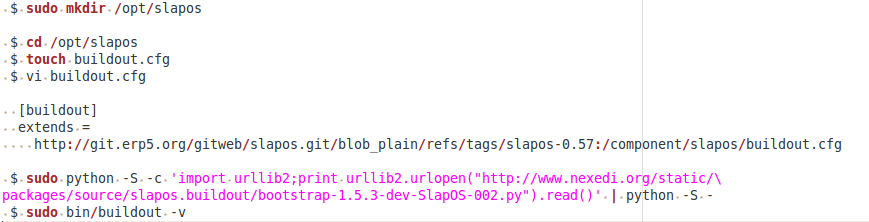
\includegraphics{figuras/slapos-1}}
    \caption{Primeira parta da instalação do SlapOS}
    \label{slapos-1}
\end{figure}

Com o termino do \textit{bootstrap} e o \textit{ script bin/buildout} é feita a instalação do SlapOS.

Após a instalação basica dos componentes e dependências é preciso configurar o mesmo, na figura \ref{slapos-2}, existe um exemplo de arquivo de configuração e logo em seguida na figura \ref{slapos-rede}, é feita a configuração de rede para uso do SlapOS, é necessário que o \textit{slapproxy} seja iniciado e mantido rodando, ele representa funcionalidades do \textit{master} do SlapOS.

\begin{figure}[ht]
    \centering
    \scalebox{0.7}{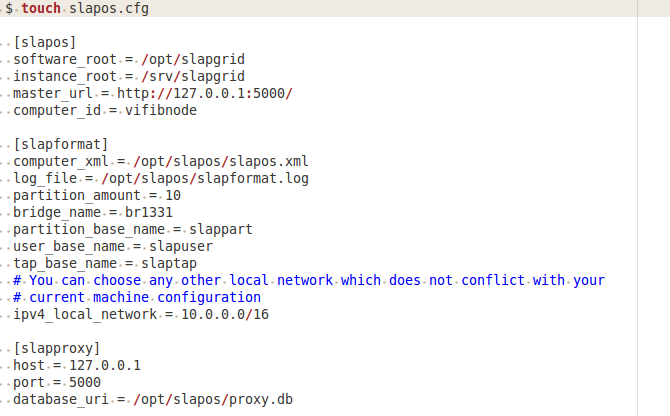
\includegraphics{figuras/slapos-2}}
    \caption{arquivo de configuração do SlapOS}
    \label{slapos-2}
\end{figure}

\begin{figure}[ht]
    \centering
    \scalebox{0.7}{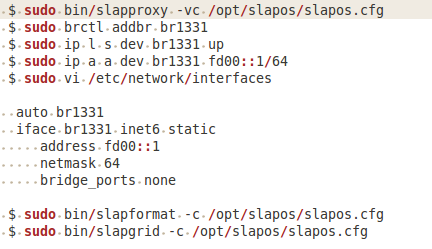
\includegraphics{figuras/slapos-rede}}
    \caption{Configurações de rede do SlapOS}
    \label{slapos-rede}
\end{figure}

É valido recordar que o SlapOS é uma ferramenta já adaptada ao IPV6, e é necessário adicionar uma configuração extra ao \textit{script /etc/network/interfaces} para habilitar as funcionalidades IPv6 do SlapOS. Por fim nas duas ultimas linhas da figura \ref{slapos-rede} são executados os \textit{scripts slapformat e slapgrid}, eles são responsáveis por registrar seu computador e devidos \textit{slots} e por habilitar o cliente SlapOS em seu computador, respectivamente.

\subsubsection{Instalação do CloudOoo}

Após realizada a instalação do SlapOS, o passo de instalação de ferramentas através do mesmo é consideravelmente simples.

Para requerer a instalação do CloudOoo é necessário utilizar o \textit{slapconsole}, assim através do mesmo e uma instância do SlapOS(\textit{slap}), referenciada na terceira linha da figura \ref{requisicao-software}, assim como no uso do \textit{bootstrap}, esta instalação também aponta para um link que é carregado e compilado.

\begin{figure}[ht]
    \centering
    \scalebox{0.7}{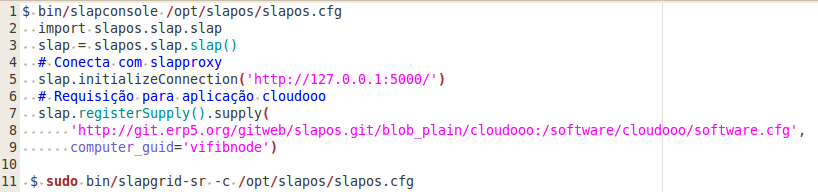
\includegraphics{figuras/requisicao-software}}
    \caption{Requisição de instalação do CloudOoo no SlapOS}
    \label{requisicao-software}
\end{figure}

Nesta referência em particular o ponteiro esta voltado para o \textit{branch} do CloudOoo, em função de suas configurações próprias que não foram encorporadas ao projeto do SlapOS.

Por fim para que ocorra a instalação dos componentes e dependências é utilizado o \textit{script slapgrid-sr}.

Após a instalação é necessário requerer uma instância, o que também ocorre pelo uso do \textit{slapconsole} de forma praticamente identica a instalação, no entanto é necessário fornecer um título a sua instância e é possível verificar se a mesma foi criada requerindo seu \textit{id}.

\begin{figure}[ht]
    \centering
    \scalebox{0.7}{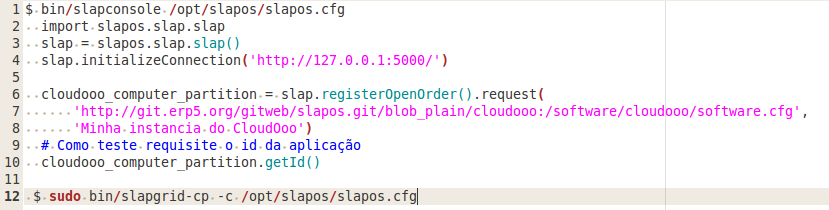
\includegraphics{figuras/requisicao-instancia}}
    \caption{Requisição de uma instância do CloudOoo via SlapOS}
    \label{requisicao-instancia}
\end{figure}

Por fim é utilizado o \textit{script slapgrid-cp} para que a criação da instâcia ocorra e seja finalizada. Após o uso da mesma será iniciado um servidor do CloudOoo pelas configurações estabelecidas no software.

\subsection{Instalação do CloudOoo.git}

Esta segunda instalação foi criada para ser mais flexível aos projetos do NSI que também utilizam o CloudOoo. Ela esta disponível no Github do NSI, em \url{http://github.com/nsi-iff/cloudooo_buildout.git}, e possui um README com instruções para instalação. Além disso esta instalação esta orientada a fazer download do repositório igualmente disponível no Github do NSI, em \url{http://github.com/nsi-iff/cloudooo}.

São necessárias apenas duas instruções para esta instalação, presentes na figura \ref{buildout-cloudooo}:

\begin{figure}[ht]
    \centering
    \scalebox{0.7}{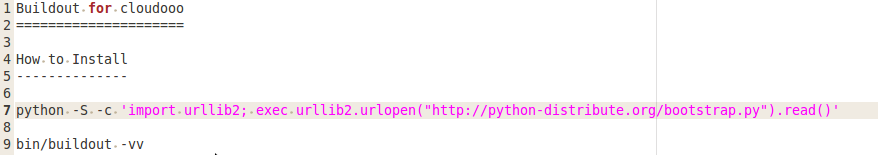
\includegraphics{figuras/buildout-cloudooo}}
    \caption{README do buildout do CloudOoo, disponível em \url{http://github.com/nsi-iff/cloudooo_buildout}}
    \label{buildout-cloudooo}
\end{figure}

Na primeira etapa utiliza-se o Python para fazer download e rodar o \textit{script} do \textit{boostrap.py}, este irá fazer o download e instalação dos componentes necessários para gerar o buildout. 

Ao termino da primeira, com o \textit{script bin/buildout} acrescido de argumentos para torná-lo verboso e do arquivo padrão de instalação(\textit{buildout.cfg}), ocorre a instalação do CloudOoo e todos os componentes necessários, entre ele o LibreOffice, FFMPEG, ImageMagick e demais.

Diferentemente da instalação via SlapOs o servidor do CloudOoo não fica disponível automaticamente para uso, é preciso ainda utilizar o \textit{script bin/supervisord}.

\section{Processos de requisições}

Para estabelecer conexão entre um cliente qualquer e o CloudOoo é necessário o uso de uma biblioteca XMLRPC. Na figura \ref{conexao} foi realizado um exemplo de cada requisição básica disponível para todos \textit{handlers}, através de uma conexão estabelecida pela biblioteca \textit{xmlrpclib}:

\begin{figure}[ht]
    \centering
    \scalebox{0.7}{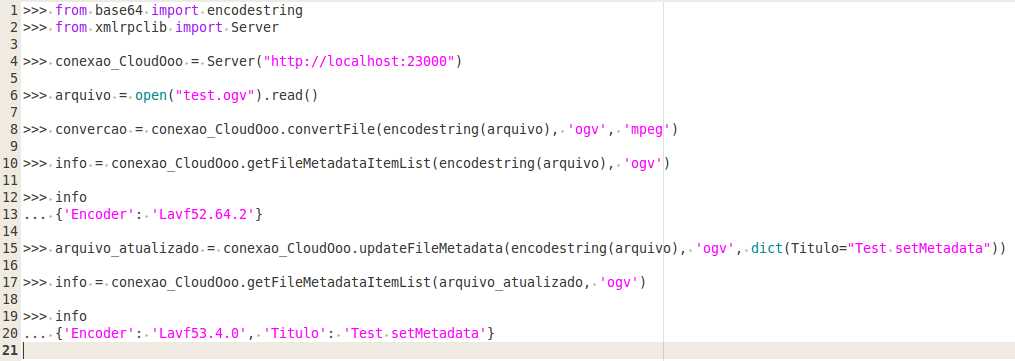
\includegraphics{figuras/conexao}}
    \caption{Exemplo prático de uso do CloudOoo}
    \label{conexao}
\end{figure}

Na linha 6 da figura a variável \textit{arquivo} recebe o conteúdo do arquivo \textit{test.ogv}, no entanto para conversão do mesmo, na linha 8, é preciso codificá-lo para que durante a passagem do cliente para o servidor esse arquivo não seja danificado, esta codificação  realizada pelo uso da biblioteca \textit{base64}.

No momento da conversão o servidor vai receber os dados do cliente, vai decodificar o arquivo e identificá-lo como um arquivo de vídeo, sendo assim o mesmo será encaminhado para o \textit{FFMPEGHandler}, que por sua vez irá convertê-lo para o formato \textit{mpeg}.

o \textit{FFMPEGHandler} também será o responsável pelos métodos de \textit{getFileMetadataItemList} e \textit{updateFileMetadata}, nos quais serão realizados respectivamente a extração e inserção de \textit{metadados} no arquivo.

Observe também que na segunda extração de \textit{metadados}, linha 17, foi utilizado o \textit{arquivo-atualizado} , resposta da requisição de inserção de \textit{metadados}, linha 15, de forma direta. Isto porque esta requisição do CloudOoo retorna um arquivo com os dados inseridos no mesmo, e que já se encontra codificado para transporte.

Além destas requisições comuns a todos os \textit{handlers} existem também requisições que foram previamente implantadas apenas para documentos:

\begin{itemize}
    \item{getAllowedExtensionList: retorna extensões permitidas para determinado arquivo;}
    \item{getChapterItem: retorna o capítulo selecionado do documento;}
    \item{getChapterItemList: retorna todos capítulos do documento;}
    \item{getColumnItemList: retorna colunas da tabela selecionada;}
    \item{getImage: retorna imagem selecionada;}
    \item{getImageItemList: retorna lista de imagens em documento;}
    \item{getLineItemList: retorna lista de linhas da tabela selecionada;}
    \item{getParagraph: retorna parágrafos selecionado;}
    \item{getParagraphItemList: retorna lista de parágrafos de um documento;}
    \item{getTable: retorna tabela selecionada;}
    \item{getTableItemList: retorna lista de tabelas no documento;}
    \item{system.listMethod: retorna lista de métodos disponíveis no servidor.}
\end{itemize}

\section{Uso do CloudOoo na Biblioteca Digital}

Para disponibilizar seu acervo, a Biblioteca Digital tem como regra converter os arquivos recebidos seu formato livre compatível, para isso utiliza de requisições ao CloudOoo. Na figura \ref{submeter-bd}, existe um exemplo de submissão de arquivos, do tipo ???, o qual passára pela conversão através de uma requisição ao CloudOoo:

\begin{figure}[ht]
    \centering
    \scalebox{0.7}{\includegraphics{figuras/submeter-bd}}
    \caption{Pagina de submissão de documentos da Biblioteca Digital}
    \label{submeter-bd}
\end{figure}

Na figura não é implicito o uso da ferramenta, uma vez que essa requisição só é realizada por formatos não livres. Outra funcionalidade implicita é a ``granularização'' realizada igualmente pelo CloudOoo. Desmonstrada na figura \ref{granulate}:

\begin{figure}[ht]
    \centering
    \scalebox{0.7}{\includegraphics{figuras/granulate}}
    \caption{Pagina de submissão de documentos da Biblioteca Digital}
    \label{granulate}
\end{figure}

Os grãos extraidos pelo processo de ``granularização'' são separados em imagens e tabelas ???, e dispostos para visualização do usuário.

\section{Performasse}

Para estabelecer a performasse o os antecessores do CloudOoo foi realizado um teste em ambos, neste teste 3699 documentos no formato odt foram selecionados, entre eles alguns documentos inválidos e outros em formatos desconhecidos. Por ser a conversão mais utilizada, foi decido que neste teste os documentos seriam convertidos para PDF.O teste foi realizado por meio do uso de \textit{script}, neles além de prover a conversão também era provido o armazenamento do tempo de cada conversão, bem como o tempo total que todas as conversões levaram em ambos.

Ao final do teste notou-se que o OOOD 2.0 levará mais tempo para realizar as conversões separadamente, no entanto com o uso excessivo ele se mostrou mais estável e mais rápido, levou 10 horas para realizar o teste e apresentou 12 erros, enquanto o OOOD 1.0 apresentou 531 erros e levou 11 horas para realizar o teste.

Para testar a performasse do CloudOoo 1.24 foram escolhidos dois testes distintos, primeiramente a repetição do teste anterior com 3699 documentos odt convertidos para PDF, para reanalisar sua performasse após suas mudanças e por segundo um novo teste com 3500 arquivos distintos sendo todos convertidos para formatos abertos equivalentes aos seus tipos específicos.

[resultado dos testes] ???

\section{Processo de Desenvolvimento}

Para \cite{PRESSMAN}, a garantia da qualidade de software de esta diretamente ligada ao emprego de testes sobre o mesmo, onde esses testes representam a expectativa do usuário sobre a aplicação, e podem ser empregados de forma automatizada ou manual. Embora testes automatizados tendam a gastar mais tempo em relação a programação dos mesmos, sua cobertura sobre o produto garante menor porcentagem de erros quando executada a aplicação.

Desde o inicio de parceria de desenvolvimento do CloudOoo tem sido aplicada a técnica chamada TDD(\textit{Test-Driven Development}), ou desenvolvimento orientado a testes, nela é defendido o desenvolvimento dos testes antes do desenvolvimento da parte funcional da aplicação, dado que os testes também fazem parte da mesma.

Segundo \cite{ASTELS}, projetos que utilizam TDD devem possuir uma suíte exaustiva de testes que por sua vez determinam o código que deve ser escrito. No entanto para uma aplicação de serviço web, existe certo grau de dificuldade de começar do zero apenas com testes, tendo por justificativa suas dependências como outras aplicações bem como a rede utilizada por este. Mesmo assim desde a parceria implementada ao CloudOoo anteriormente, até seu estado atual seu desenvolvimento tem partido do principio de realizar testes antes de implementar suas funcionalidades. Isto porque, além da garantia de qualidade, o uso de testes nele serviu de auxilio ao desenvolvimento dado todos as configurações que devem ser estabelecidas para funcionamento deste. Entre elas o próprio padrão das aplicações externas que não estão ligadas diretamente ao sistema operacional do servidor e que precisam ser apontadas por meio de \textit{scripts}.

Além do testes, outra ferramenta que garante o desenvolvimento do CloudOoo é o uso de sistemas de controle de versão, como o \textit{subversion}, que era utilizado na versão 2.0, e que atualmente foi trocado pelo \textit{git} em função de suas diversas vantagens como o controle de versões distribuído por exemplo. A importância do controle de versão esta no controle do crescimento desta aplicação, que por momentos contou com uma equipe de desenvolvimento sem contato constante, assim por meio de ferramentas como estas podiam acompanhar as modificações da aplicação, bem como reverter determinadas alterações em casos de erros posteriores na mesma.

Sob certo ponto de vista o uso destas práticas sugere sobre o desenvolvimento do CloudOoo severas semelhanças com os métodos ágeis, muito embora não exista a definição propriamente dita de nenhuma delas aplicadas diretamente sobre o projeto.

Em seu artigo \cite{SILVA-MONNERAT-CARVALHO}, comprovam o uso do TDD no CloudOoo, e de suas complicações de emprego, uma vez que inicialmente não existia total proficiência por parte dos desenvolvedores. Além disso foi verificado sobre o estabilidade do desenvolvimento do projeto, tomando por base a lista de mudanças armazenadas pelo controle de versão. Observou-se através deste artigo que embora no incio do projeto nenhum teste falhasse, conforme o mesmo foi acrescido de mudanças e novas funcionalidades testes que antes passavam passaram a apresentar erros antes não conhecidos, precisando assim de correções.

Estas implicações trazem ao meio de software uma compreensão muito similar ao do ramo de indústria, no que se desrespeita a aplicação de novas técnicas para garantir que quando um produto chega ao meio de produção possa continuar estável ao uso.
